\chapter{Funktionelle krav}\label{Funktionellekrav}
De funktionelle krav beskriver de funktioner, systemet skal have. Kravene er beskrevet ved hjælp af use cases, der bl.a. beskriver, hvordan en aktører anvender systemet til at opnå et mål. Figur \ref{UseCaseDiagram} viser et use case diagram, som illustrerer den enkeltes aktørs interaktion med de de forskellige use cases. 

\section{Use Case Diagram}
\begin{figure}[H]
    \centering
    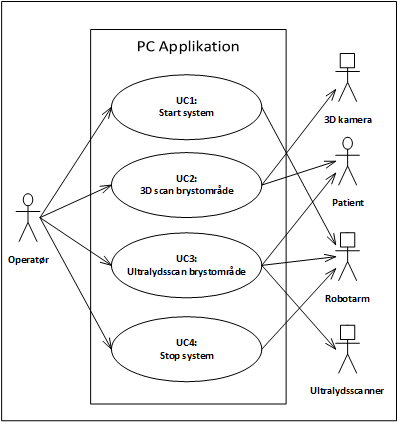
\includegraphics[width=0.80\textwidth]{figurer/d/Kravspecifikation/UseCaseDiagram}
    \caption{Use Case Diagram}
    \label{UseCaseDiagram}
\end{figure}
\newpage

\section{Fully-dressed Use Cases}
Hver use case (UC) er beskrevet med et mål, interagerende aktører, hvad der initerer use casen, forudsætningen, resultat og forløbet i use casen. Målet beskriver, hvad der ønskes opnået, mens resultatet beskriver, hvad systemet har gjort ved slutningen af use casen. 

Efter afsluttelse af UC1: Start system, vil det til en hver tid være muligt at afbryde den igangværende use case, og dermed starte UC4: Stop system.

\subsection{Use Case 1}
\begin{longtabu}{ | l | p{0.8\textwidth} | }
  \hline
  \multicolumn{2}{|c|}{\textbf{UC1: Start system}} \\ \hline
  \textbf{Mål} & At forberede scanninngen \\ \hline
  \textbf{Aktører} & Operatør, Robotarm \\ \hline
  \textbf{Initiering} & Operatør  \\ \hline
  \textbf{Forudsætninger} & Computer, der skal køre PC Applikation, er tændt. Robotarm er tilsluttet  \\ \hline
  \textbf{Resultat} & PC Applikation er startet \\ \hline
  \textbf{Hovedforløb} & 
  	{\begin{enumerate}
  	\item Operatør starter PC Applikation ved at klikke på 'AutoSonography.exe' på computerens skrivebord
  	\item PC Applikation instruerer Robotarm tilbage til standardposition
  	\end{enumerate}} \\ \hline
\end{longtabu}
\newpage

\subsection{Use Case 2}
\begin{longtabu}{ | l | p{0.8\textwidth} | }
  \hline
  \multicolumn{2}{|c|}{\textbf{UC2: 3D scan brystområde}} \\\hline
  \textbf{Mål} & At konstruere et dybdebillede af Patients brystområde, så UC3: Ultralydsscan brystområde kan begyndes  \\\hline
   \textbf{Aktører} & Operatør, Patient, 3D kamera \\\hline
  \textbf{Initiering} & Operatør  \\\hline
  \textbf{Forudsætninger} & UC1: Start system  er gennemført. 3D kamera er tilsluttet computeren. Patients brystområde er indenfor afgræsning, mens Patients hoved og arme er udenfor afgrænsning \\\hline
  \textbf{Resultat} & Patients brystområde er blevet scannet af 3D kamera \\\hline
  \textbf{Hovedforløb} & 
  	{\begin{enumerate} 
  	\item Operatør trykker på knappen [3D Scan] på GUI's Startup Menu
  	\item Operatør trykker på knappen [Scan] på GUI's 3D Scan Menu
	\begin{itemize}
	\item \textit{'Juster 3D billedets skæring'}  	
  	\end{itemize} 
  	\item PC Applikation instruerer 3D kamera til at scanne brystområde på Patient
  	\item Operatør godkender dybdebilledet på knappen [OK] på GUI's 3D Scan Menu efter efter endt scanning 
	\begin{itemize}
	\item \textit{'Dybdebillede er forvrænget '}  	
  	\end{itemize} 
  	\end{enumerate}} \\\hline
   \textbf{Undtagelser} &   
  	{\begin{itemize} 
  	\item \textit{'Juster 3D billedets skæring'}
  	\begin{enumerate}[label=A\arabic*]
		\item Operatør vælger et andet skæringsinterval på GUI for Patients brystområde
		\item Operatør forsætter UC2: 3D scan brystområde
	\end{enumerate}
  	\item \textit{'Dybdebilledet er forvrænget'}
  	\begin{enumerate}[label=B\arabic*]
		\item Operatør godkender ikke billedet og trykker på knappen [Scan] 
		\item Systemet genstarter UC2: 3D scan brystområde
	\end{enumerate}
	\end{itemize}} \\\hline
	\end{longtabu}
\newpage

\subsection{Use Case 3}
\begin{longtabu}{ | l | p{0.8\textwidth} | }
  \hline
  \multicolumn{2}{|c|}{\textbf{UC3: Ultralydsscan brystområde}} \\ \hline
  \textbf{Mål} & At få en ultralydsscanning af Patients brystområde \\ \hline
   \textbf{Aktører} & Operatør, Robotarm, Ultralydsscanner \\ \hline
  \textbf{Initiering} & Operatør \\ \hline
  \textbf{Forudsætninger} & UC2: 3D scan brystområde er gennemført. Patient har ikke skiftet position fra UC3: 3D scan brystområde.  Ultralydsscanner er tændt. Robotarm  er tændt og tilsluttet  \\ \hline
  \textbf{Resultat} & PC Applikation har instrueret Robotarm i at flytte Ultralydsscanner omkring Patients brystområde således, at der konstrueres en ultralydsscanning \\ \hline
  \textbf{Hovedforløb} & 
  	{\begin{enumerate} 
  	\item Operatør trykker på knappen [Ultralyddscan] på GUI's Startup Menu
  	\item PC Applikation benytter 3D kameras dybdebillede fra UC2: 3D scan brystområde til at instruere Robotarm til ny positur, for at bevæge Ultralydsscanner på Patient
  	  	\begin{itemize}
  	  	\item \textit{'Operatør pauser scanning'}
  		\item \textit{'Operatør stopper scanning'}
  		\end{itemize}
  	\item PC Applikation instruerer Robotarm tilbage til standardposition
  	\end{enumerate}} \\ \hline
  	\textbf{Udvidelser} & 
  	{\begin{itemize} 
  	\item \textit{'Operatør pauser scanning'}
  		\begin{enumerate}[label=A\arabic*]
  		\item Operatør trykker på knappen [Pause] på GUI's Ultralydsscan Menu, og PC Applikation stopper Robotarm indenfor 5 sekunder
  		\item Operatør trykker på knappen [Pause] på GUI's Ultralydsscan Menu, og Robotarm genoptager scanningen indenfor 2 sekunder   		
  		\end{enumerate}
  	\end{itemize}} \\ \hline
  \textbf{Undtagelser} & 
  	{\begin{itemize} 
  	\item \textit{'Operatør stopper scanning'}
  		\begin{enumerate}[label=B\arabic*]
  		\item Operatør trykker på knappen [Stop] på GUI's Ultralydsscan Menu
  		\item PC Applikation instruerer Robotarm tilbage til standardposition
  		\end{enumerate}
  	\end{itemize}} \\\hline
\end{longtabu}

\subsection{Use Case 4}
\begin{longtabu}{ | l | p{0.8\textwidth} | }
  \hline
  \multicolumn{2}{|c|}{\textbf{UC4: Stop system}} \\ \hline
  \textbf{Mål} & At stoppe systemet \\ \hline
  \textbf{Aktører} & Operatør, Robotarm \\ \hline
  \textbf{Initiering} & Operatør\\ \hline
  \textbf{Forudsætninger} & UC1: Start system er færdiggjort. Robotarm  er tændt og tilsluttet  \\ \hline
  \textbf{Resultat} & PC Applikation er lukket ned og Robotarm er i standardposition\\ \hline	
  \textbf{Hovedforløb} & 
  	{\begin{enumerate}
  	\item Operatør lukker softwaren ved at trykke på knappen [Luk] på GUI's Startup Menu
  	\item PC Applikation instruerer Robotarm tilbage til standardposition
  	\end{enumerate}} \\ \hline
\end{longtabu}